\chapter{Development of a numerical landscape evolution model for high-performance computing}
\label{chapter_HAIL-CAESAR}
\chaptermark{A landscape evolution model for HPC}

%\begin{chapquote}{The GNU gcc compiler \textit{}}
%``Segmentation fault.''
%\end{chapquote}


\section{Introduction}
Computer-based numerical models of landscapes have evolved since their introduction in the late 1970s, \citep[e.g.,][]{ahnert1976quantitative} to a point where they are now used to investigate a range of interacting processes in landscape systems including catchment hydrology, sediment transport, hillslope mass movement, and biological processes \citep{Pazzaglia2003,Willgoose2005,Tucker2010}. Such models have developed over time to become useful tools not only for understanding how landscapes have formed in the past, but also how they will evolve in the future, such as in response to climatic or environmental change \citep{bras2003six, church2003geomorphological, pelletier2015forecasting}. Landscape evolution models, as they are often collectively termed, enable catchment scientists, hydrologists, and geomorphologists to investigate landscape change on a range of timescales and spatial resolutions. They address societal needs to forecast the landscape's response to environmental change, as well as further the understanding of individual geomorphological processes and their interaction in forming whole landscapes \citep{dietrich2003geomorphic}.

The data driving landscape evolution models, such as the digital elevation models (DEMs) used to represent the landscape surface, and other inputs such as climatic data, have increased rapidly in spatial resolution in recent years \citep[e.g.,][]{gesch2002national, rabus2003shuttle, tarolli2009understanding, casas2006topographic, krishnan2011opentopography}. Topographic datasets have increased in resolution to sub-metre scales, particularly since the advent of terrestrial LiDAR-derived digital elevation models, which are now a common data source in geomorphological analyses and modelling studies \citep{bates2003optimal, passalacqua2010geometric,clubb2014objective}. The growth of high resolution input data is a double-edged sword: it presents the numerical modeller with the opportunity of studying processes at finer scales, often allowing sub-grid processes such as channel morphology to be resolved at the grid-cell scale \citep{schoorl2000three}. However, higher-resolution data also increases the computational cost of model simulations, as the number of calculations at a given model timestep increases with increasing number of grid cells used to represent the model domain. Decreasing the grid cell size of an input dataset causes the total problem size -- the number of grid cells in the model domain -- to increase non-linearly. Rising demand to study landscape and catchment processes at a regional or even continental scale also increases the computational cost of a model simulation by increasing the total number of grid cells in a model domain. Process representation has also grown in complexity, with many LEMs now supporting a range of rainfall-runoff, flow routing, erosion and slope process laws in a single model \citep{Coulthard2001, Tucker2010, hobley10creative}, further increasing the computational demands made by modelling studies. 

% link into to advent of hpc systems here?
Rapid growth in computing power has occurred in tandem with the computational demands made by the hydrological and landscape evolution modelling communities. Individual processor power has steadily increased in following with the predictions made by Moore's law \citep{schaller1997moore, moore1998cramming}, through a continued increase in the number of transistors on integrated circuitry. As the rate of increase in individual processor speed has slowed in recent years \citep{mann2000end,colwell2013chip}, parallel processing -- the use of multiple processors to tackle larger computational problems --  has become a indispensable tool in the scientific computing community. The uptake of parallelisation methods by the numerical landscape evolution modelling community is still in its infancy \citep{valters2016modelling}. However, disciplines with a close affinity to geomorphology have explored the use of parallel computing technologies in order to study larger problem sets, such as in the hydraulic modelling community \citep[e.g.,][]{ivanov2004catchment, neal2009parallelisation, kollet2010proof, smith2013towards, liang2015high,smith2015towards}. The increasing demand for environmental model codes capable of exploiting the parallelism offered by high-performance computing technologies has lead to the development of the HAIL-CAESAR landscape evolution model. 

This paper presents an implementation of the CAESAR-Lisflood model \citep{Coulthard2013}, re-written and adapted to be compatible on for shared-memory parallel computing environments. The version presented here, termed HAIL-CAESAR\footnote{High-performance Architecture Independent Lisflood-CAESAR model, where \textit{CAESAR} was originally the Cellular Automaton Evolutionary Slope and River model}, provides an operating-system independent, open source, hydrodynamic landscape evolution model suitable for deployment on various computing environments, including high performance computing architectures.


\section{Model description and parallelisation}

\subsection{Origins: CAESAR-Lisflood}
The porting and modifcation of HAIL-CAESAR is based on the CAESAR-Lisflood model \citep{Coulthard2013}, a cellular automaton numerical model of landscape evolution integrated with a hydrodynamic flow model \citep{bates2010simple}. CAESAR-Lisflood is an open-source, GUI-based landscape evolution model written in the C\# programming language, and distributed as a  Windows\texttrademark  \ executable file. As of version 1.9b \citep{coulthard2017caesarlisflood}, there was no platform-independent version of the code, and users are required to run the model in GUI-mode on a Windows-based desktop computer. The model was therefore unsuitable for running on Unix-based operating systems, such as those typically found on cluster computing facilities. High performance computing systems, beyond those of typical desktop computers, could not be taken advantage of to run computationally expensive simulations. 

\subsection{HAIL-CAESAR}

HAIL-CAESAR, much like the original CAESAR-Lisflood model it is based upon, is a cellular automaton, landscape evolution model for simulating hydrological and sediment transport processes at the river catchment scale. The key components of the model are a hydrodynamic water flow-routing model, and a sediment erosion and transport model (Figure \ref{fig_flowchart}). The model is designed to simulate catchment processes on timescales of hours, years, and hundreds of years. The HAIL-CAESAR model is an open source, platform-independent C++ implementation of the algorithms in the CAESAR-Lisflood model described in the next section. The model is run from a command line or terminal interface, with the user supplying a parameter file that initialises the variables within the model, and specifies the supplementary input files such as terrain DEM and rainfall input data. The user controls the majority of the model's operation by changing the parameter file variables. An outline of the program flow, file inputs and outputs is shown in Figure \ref{fig_flowchart}.

\paragraph*{Object-oriented framework}
The HAIL-CAESAR model is designed within an object-oriented framework, enabling more advanced users to make modifications to the general model structure (Figure \ref{fig_flowchart}) by modifying the supplied \textit{HAIL-CAESAR-driver.cpp} file. The modular approach to the model's functionality allows advanced users to create their own custom versions of the model in a structured way using object-oriented principles. The model is also integrated with the LSDTopoTools topographic analysis framework, a C++ software package for the analysis and modelling of landscapes using raster input data. In the object-oriented framework, model simulations are created as object instances, and then methods can be called upon the model object, for example:

\begin{verbatim}

LSDCatchmentModel mySim("parameters.txt")
// Create an instance of the model 
// using an input parameter file.

mySim.loaddata();
mySim.water_inputs(); 
mySim.depth_update(); 
mySim.flow_route(); 
mySim.erode(); 

\end{verbatim} 

The flexibility of the object-oriented framework allows the user finer control over the complexity of the simulation in terms of process representation, adding and removing landscape processes as necessary. This modularity in landscape evolution modelling codes is also seen in the CHILD \citep{Tucker2001} and Landlab \citep{hobley10creative} modelling frameworks.
%\paragraph*{Fully distributed hydrology}
%
%\paragraph*{Interoperability with netCDF data}

\subsection{Process representation}

\subsubsection{Catchment hydrology}

Runoff from rainfall inputs to the catchment is generated using an adaptation of the TOPMODEL hydrological model \citep{beven1979physically}. The TOPMODEL approach first calculates a combined surface and subsurface discharge for the cells within a `wetted' zone of the catchment \citep{coulthard2002cellular}. The wetted cells approach has the advantage of reducing the number of cells that must be scanned every model iteration, lowering computational cost of the model run. When local rainfall rate in a given grid cell is greater than zero, the total runoff, \(Q_{tot}\), for a grid cell is given by: 

\begin{equation}
Q_{tot} = \frac{m}{T} \log \left( \frac{(r-j_t) + \exp \left(\frac{rT}{m} \right)}{r} \right)
\end{equation}
where \(m\) is a parameter that controls the rise and fall of the soil moisture store, \(j_t\), \(T\) is the time step in seconds, and \(r\) the rainfall rate in metres per hour. The soil moisture store, \(j_t\), is given by the formula:

\begin{equation}
j_t = \frac{r}  { \left(  \frac{r-j_{t-1}}{j_{t-1}  } \exp \left( \left( \frac{(0-r)T}{m}\right) +1 \right) \right)}
\end{equation}

\noindent
When rainfall rate is zero during the current iteration, the total runoff, \(Q_{tot}\), is given by the equation:

\begin{equation}
Q_{tot} =  \frac{m}{T} log \left( 1 + \left( \frac{j_t  T}{m} \right) \right)
\end{equation}

\noindent
with the soil moisture store, \(j_t\), given by:

\begin{equation}
j_t = \frac{j_{t-1}}{1 + \left( \frac{j_{t-1}T}{m} \right) }
\end{equation}

\noindent
Total runoff, \(Q_{tot}\), is apportioned between surface and subsurface discharge by a user-set threshold for discharge, \(Q_{min}\). When the volume of water for a given cell exceeds this threshold, it is treated as surface runoff and routed according to the flow routing algorithm described in the following section.

%

\subsubsection{Surface flow routing}
Surface water and channel flow is an important driver of catchment scale erosional processes. The amount and velocity of water flow is a variable in both the sediment transport and bedrock erosion laws. The surface water flow equations are based on a simplified form of the shallow water flow equations, a simplification first derived by \citet{bates2010simple} and later incorporated into the CAESAR-Lisflood landscape evolution model by \citet{Coulthard2013}. The flow between cells is calculated by:

\begin{equation}
Q = \frac{q - g h_{flow} \Delta T \frac{\Delta (h+z) }{\Delta x}}{1 + g h_{flow} \Delta t n^2 |q| / h_{flow}^{10/3}} \Delta x
\end{equation}


\subsubsection{Sediment transport and erosion}
\label{trans_model}

Transport of loose sediment is governed by the \citet{wilcock2003surface} sediment transport model. The Wilcock and Crowe model represents transport of mixed sand/gravel fractions based on the surface sediment composition. The rate of sediment transport, \(q_i\), is given as:

\begin{equation}
q_i = \frac{F_i {U_*}^3 {W_i}^*}{(s -1) g}
\end{equation}

\noindent
where \(F_i\) is the fractional volume of sediment, for a given sediment fraction, \(i\), \(U^*\) is the shear velocity, \(s\) is the ratio of sediment to water density. \({W_i}^*\) is a function relating fractional transport rate to total transport rate \citep[see][for a full derivation of this equation]{wilcock2003surface}. The usage of this sediment transport model is extrapolated here to account for finer particles such as silts \citep{van2007embedding}, as well as the sand-gravel mixture it was originally designed for.

\subsubsection{Bedrock incision}
\label{bedrock_model}
A simple model of bedrock incision based on the excess shear stress model \citep{tucker2001child,tucker2004drainage} is implemented in the numerical model. The rate of bedrock incision is determined by the amount of shear stress acting on the bedrock, above a threshold level of stress required to initiate substrate removal \citep[e.g.,][]{Snyder2003}. When bedrock material is removed, it is distributed amongst the sediment fractions according to the fractional proportions set by the user. The rate of bedrock erosion according to the excess shear stress model is given by:

\begin{equation}
\varepsilon = k_e(\tau_b - \tau_c)^{P_b}
\end{equation}

\noindent
where \(k_e\) is the bedrock erodibility coefficient, \(\tau_b\) is the basal shear stress on the channel bed, \(\tau_c\), is the critical shear stress threshold, \(P_b\) is the shear stress exponent \citep{howard1983channel,whipple1999dynamics}.

\subsection{Parallelisation implementation}
The HAIL-CAESAR code is parallelised using a shared-memory parallelisation model. In brief, the shared-memory technique works by distributing the processing load to multiple processing units that all have access to the same memory address space. The HAIL-CAESAR code uses the OpenMP application programming interface (API), which is widely supported on a range of software platforms and computing architectures \citep{dagum1998openmp}. Shared-memory parallel codes such as the one described in this paper are suitable for any computing system where the physical processors have access to the same memory space. A wide range of systems can avail of shared-memory parallel codes, from multi-core desktop computers, through high-end multi-processor, multi-core workstations, to individual compute nodes on high performance computing services (HPC). The code presented has been tested on a wide range of architectures including desktop computers,  small-scale cluster computing facilities, and national scale HPC services.

The main functions in the program that are parallelisable, and most computationally expensive, are the water routing algorithm (\textit{flow\_route}), the erosion routines (\textit{erode}), the water depth update function (\textit{depth\_update}), and the catchment wetted-area scanning function (\textit{scan\_area}). These were identified by profiling the serial version of the code using the \textit{gprof} profiling tool \citep{graham1982gprof}, and the results are shown in Tables \ref{profile_speed_up_hydro} and \ref{profile_speed_up_erode}. Initially, it may appear that using a wetted-cells approach with the \textit{scan\_area} function would be a counter-intuitive way to reduce computation time, as the \textit{scan\_area} function is computationally expensive itself. However, preliminary experimentation with removing the \textit{scan\_area} function (and scanning all cells in the catchment every iteration) showed that in fact the computational expense of calling this function was far outweighed by the large reduction in cells that had to be scanned every iteration. In practice this is likely due to the fact that catchments are rarely inundated totally, even during flood events, as only the floodplains maintain a significant depth of water. The number of wetted cells is therefore likely to be much smaller than the total number of grid cells in the model domain for the majority of cases, and the wetted cell scanning function (\textit{scan\_area}) overall reduces computation time.

\begin{table}
\caption{Summary of most expensive program functions, using a test case of a 48 hour flood simulation, with the model run in \textbf{hydrology-only mode}. The test case is based on the flooding that took place in the Boscastle catchment in August 2004, in Cornwall, UK \citep{golding2005boscastle}.}
\begin{tabular}{cl}
%\multicolumn{2}{c}{\textbf{Profiling results of 48 hour simulation in hydrological mode}} \\

\textbf{Time} (percentage of total) & \textbf{Function name} \\
\hline
77.71                                     & flow\_route \\
17.63                                     & depth\_update \\
3.58                                       & scan\_area \\
1.02                                       & catchment\_waterinputs \\
0.03                                       & water\_flux\_out \\
\hline \\
\end{tabular} 
\label{profile_speed_up_hydro}
\end{table}

\begin{table}
\caption{Summary of most expensive program functions, \textbf{with erosion processes enabled}, using a test case of a 48 hour flood simulation. The test case is based on the flooding that took place in the Boscastle catchment in August 2004, in Cornwall, UK \citep{golding2005boscastle}.}
\begin{tabular}{cl}
%\multicolumn{2}{c}{\textbf{Profiling results of 48 hour simulation in erosion-enabled mode}} \\

\textbf{Time} (percentage of total) & \textbf{Function name} \\
\hline 
37.96                                    & erode \\
25.68                                     & flow\_route \\
15.90                                       & scan\_area \\
11.47                                      & depth\_update \\
3.75                                    & (matrix library functions) \\
1.84                                       & d50 \\
1.63                                       & slide\_GS \\
0.59                                      & sort\_active \\
0.46                                      & catchment\_waterinputs \\
0.20                                     & sand\_fraction \\
\hline \\
\end{tabular} 
\label{profile_speed_up_erode}
\end{table}


\paragraph*{flow\_route}
The \textit{flow\_route} function is the core water-routing algorithm based on the \citet{bates2010simple} algorithm. The \textit{flow\_route} function accounts for c. 26\% of compute time in a typical erosion-enabled simulation, and 78\% of compute time in a flow-only simulation.  As one of the most compute-intensive sections of code when the catchment is in flood, the parallelisation of this section achieved significant overall code speed up for a variety of data inputs. The flow routing algorithm is only performed on those cells in the model domain that have accumulated a water depth, i.e. it is not performed in `dry' cells. This means that only a small subset of cells are accessed during the flow routing section of the code, given a typical scenario where there is significant amounts of flow in the channels and floodplain areas, but little or none on the hillslopes. The code and parallelisation of the \textit{flow\_route} function is given in outline form below:

\begin{verbatim}
#pragma omp parallel for
    schedule(runtime)
for (int y=1; y<=jmax; y++)
{
  int inc = 1;
  while (down_scan[y][inc] > 0)
  {
  // Water routing in x direction...
  
  // Water routing in y direction...
  inc++;
}
\end{verbatim}

\paragraph*{depth\_update}
Profiling of the serial code identified the water depth update function as being one of the most compute intensive parts of the code for hydrology-only and erosion-enabled simulations. Updating of water depths is done using the same scanning algorithm as described for \textit{flow\_route}, updating depths in cells where there is water, or in neighbouring cells to water-containing cells. An outline of the implementation is presented below:

\begin{verbatim}
#pragma omp parallel for 
     reduction(max:l_maxdepth)
     schedule(runtime)
for (unsigned y = 1; y<= jmax; y++)
{
  int inc = 1;
  double tempmaxdepth = 0;
  while (down_scan[y][inc] > 0)
  {
    // Update water depths
    // Update suspended sediment 
    //   concentrations
    // Calculate maximum flow depth
    ...
    inc++;
  }
}
\end{verbatim}

\paragraph*{scan\_area}
The \textit{scan\_area} function analyses the catchment to determine which cells contain water or neighbour water-containing cells and sets an index array based on the current wetted area of the catchment. Further functions that involve updating sediment or water transport amounts then use this array as a mask so that only catchment model cells that contain water will be inspected and have their sediment and water totals updated.
\begin{verbatim}
#pragma omp parallel for
for (int j=1; j <= jmax; j++)
{
  int inc = 1;
  for (int i=1; i <= imax; i++)
  {
    // zero down_scan array
    down_scan[j][i] = 0;
    // and work out scanned area. 
    if (water_depth[i][j] > 0
        || water_depth[i][j - 1] > 0
        || water_depth[i][j + 1] > 0
        || water_depth[i - 1][j] > 0
        || water_depth[i - 1][j - 1] > 0
        || water_depth[i - 1][j + 1] > 0
        || water_depth[i + 1][j - 1] > 0
        || water_depth[i + 1][j + 1] > 0
        || water_depth[i + 1][j] > 0
        )
        {
        down_scan[j][inc] = i;
        inc++;
        }
    }
}
\end{verbatim}

\paragraph*{erode}
The most compute-intensive part of the code when run in erosion-enabled mode is the \textit{erode} function. This function performs all sediment entrainment and transport routines. The serial-run test simulation spent c. 38\% of its time in this function, plus an additional 5\% of time in function calls within the main \textit{erode} routine. 

\begin{verbatim}
#pragma omp parallel for 
    reduction(max:tempbedloadmax) 
    schedule(runtime) 
for (unsigned int y = 1; y < jmax; ++y) 
{
  int inc = 1;
  while (down_scan[y][inc] > 0)
  {
    unsigned x = down_scan[y][inc];
     inc++;
     // Calculate sediment entrainment
     ...
   }
}

#pragma omp parallel for
{
  // Sediment transport in x-direction
}

#pragma omp parallel for
{
  // sediment transport in y-direction
}

#pragma omp parallel for
{
  // Calculate sediment transport
  //   from all 4 edges
  // of the model domain
}

\end{verbatim}

\begin{figure}[t]
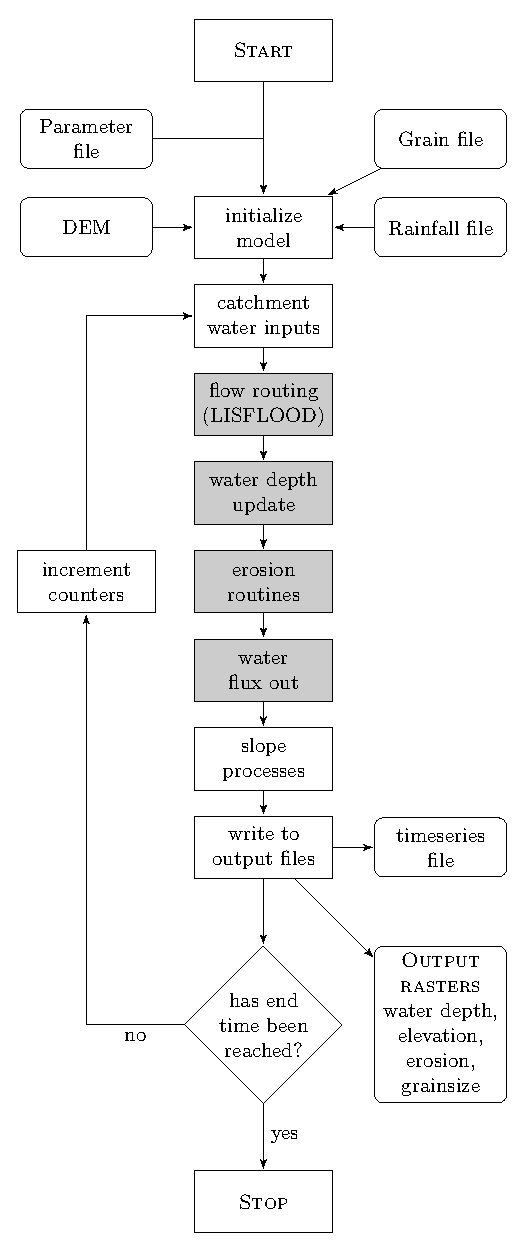
\includegraphics[width=8.3cm]{chp05_figures_scripts/tikz.eps}
\caption{Flow chart showing a simplified outline of the HAIL-CAESAR program flow. Grey shaded boxes indicate sections of the code parallelised with OpenMP. Rounded rectangles indicate output and input files.}
\label{fig_flowchart}
\end{figure}

\subsection{Potential speed up from parallelisation}

The functions described above, \textit{flow\_route, depth\_update, scan\_area,} and \textit{erode}, account for 98\% and 94\% of the compute-time in hydrology-only and erosion-enabled modes, respectively. The model is profiled using a 48 hour test simulation of a flash flood event in the summer of 2004 in the UK, referred to as the `Boscastle' simulation. (Full details of this flood event are described in Chapter \ref{chapter_events}.) Effective parallelisation of the compute-time dominating functions should result in effective parallel speed-up. The potential speed-up as a result of parallelisation can be estimated using Amdahl's law \citep{amdahl1967validity}. The law gives the predicted speed up on \(N\) processing units based on ideal scaling over multiple cores. Ideal parallel speed-up, \(S\) is given by:

\begin{equation}
S = \frac{1}{(1-P)+(P/N)}
\label{eqn_amdahl}
\end{equation}

\noindent
where \(P\) is the proportion of program time that can be run in parallel. (Note that \(P\) may vary slightly between simulations, based on the input data and certain model parameters supplied to the program.) Profiling the program with the Intel VTune amplifier performance analysis tool suggests that the program spends 94\% of its time in parallel sections of the code during an erosion-enabled simulation and 98\% of compute-time in parallel sections during a hydrology-only simulation. Using Amdahl's law it is possible to calculate theoretical potential speed-up given in Table \ref{Amdahl_table}. At the maximum available processor count of 48 cores, speed ups of up to c.20 times are predicted for a hydrology-only simulation, and up to c.13 times for an erosion-enabled simulation. The limitations of Amdahl's law are that it predicts only idealised speed ups, and does not account for any overheads in parallelisation, such as the creation and synchronisation of threads, nor does it account for performance issues due to the speed of memory access in memory-bound computational problems \citep{hill2008amdahl,sun2010reevaluating}.

\begin{table}
\caption{Idealised potential speed-up according to Amdahl's law (equation \ref{eqn_amdahl}). Value for \(P\) calculated using profiling results from the River Valency flood test simulation after 48 hours simulated time.}
\begin{tabular}{ccc}
%\multicolumn{3}{c}{\textbf{Idealised parallel speed-up}} \\ 
\textbf{Number of CPUs} & \textbf{Speed-up} (Hydro) & \textbf{Speed-up} (Erosion) \\

 & \(P=0.98\) & \(P=0.94\) \\
\hline 
2 & 1.94 & 1.89  \\ 
4 & 3.67 & 3.39  \\ 
8 & 6.11 &5.63  \\ 
16 & 11.03 & 8.42 \\ 
32 & 16.58 & 11.2 \\ 
48 & 19.92 & 13.4 \\ 
\hline \\
\end{tabular}

\label{Amdahl_table} 
\end{table}



\section{Testing and benchmarking}

Two aspects of model performance are tested in this section. Firstly, tests are carried out to verify that the HAIL-CAESAR model produces comparable scientific results with that of its progenitor, CAESAR-Lisflood. Secondly, benchmarking tests are done to measure any performance gains of HAIL-CAESAR arising from its implementation in C++, parallelisation strategy, and choice of compiler. The HAIL-CAESAR model is tested with two different compilers, to assess any potential differences arising from the choice of compiler. These are the \textit{GCC (GNU compiler collection)} C++ compiler and the \textit{Intel} C++ compiler. The CAESAR-Lisflood model is supplied already compiled with the Microsoft \textit{MSVC} C\# compiler. In all cases, compiler optimisation flags are turned on for the compilation process.

\subsection{Regression testing}

Regression testing is a software development practice used to verify that software that has been modified, interfaced with other software, or re-implemented, still performs as expected when compared to the original implementation \citep{wong1997study}. To verify that HAIL-CAESAR produces comparable results to the original CAESAR-Lisflood model, a set of simulations with the same test data and input parameters for both models is carried out. The catchment hydrological and sediment outputs from a 10-year simulation of the River Swale, North Yorkshire, United Kingdom are compared for consistency between both implementations. The Swaledale test case has been well calibrated in previous studies \citep[e.g.,][]{Coulthard2001} and is supplied with the original CAESAR-Lisflood model as a standard test case. Details of the model testing simulations are shown in Table \ref{versus_CL}. 

Three metrics are used to compare the two models (and choice of compiler in HAIL-CAESAR): water discharge rate from the catchment outlet, hourly sediment output, and cumulative sediment output from the catchment over the course of the simulation. 
Figure \ref{fig_swale_regression_lisflood} shows the differences in water discharge comparing HAIL-CAESAR with the original CAESAR-Lisflood model. (For clarity, only the first 250 days are shown.) The flow routing algorithm performs similarly in both models, with the largest discrepancies seen in the first 100 days. An inset in Figure \ref{fig_swale_regression_lisflood} shows the typical magnitude and timing of differences in the discharge. The timing and magnitude of the largest flood peaks are comparable, and the largest differences in magnitude on the order of 1--10 \(m^3s^{-1}\).
Figure \ref{fig_swale_regression_sediment} shows the sediment flux from the catchment outlet. While there is low-magnitude variation in the sediment flux signal, the main peaks in sediment discharge are at similar times and of similar magnitude in both implementations. Figure \ref{fig_swale_regression_cum_sediment} shows the cumulative sediment output from the catchment. Initially, both implementations show close agreement, until approximately 700 days into the test simulation where the predicted sediment totals begin to diverge. The CAESAR-Lisflood implementation, in this case, predicts an overall lower total sediment discharge over the 10-year period. The HAIL-CAESAR implementation predicts c. 40\% greater total sediment yields after 10 years.

\subsection{Differences in sediment flux and yields between models and compilers}

Several factors may explain the small differences seen between the sediment outputs of the two models (HAIL-CAESAR vs CAESAR-Lisflood) and also in the comparison between the two compilers used to test HAIL-CAESAR. The sediment flux differences are shown in detail for first 250 days of the Swale test simulation in Figure \ref{fig_swale_regression_sediment}.

Firstly, floating point numbers cannot be represented exactly in computer memory, due to a finite amount of memory or `bits' that may be used to store each number. In the case of these tests, a \textit{64-bit} data type is used to store numbers. Many calculations using real numbers will produce a result that cannot be represented in the finite number of bits provided by the system ($10 \div 3$, for example, results in 3.333333..., which cannot be stored precisely in a 64-bit data type, or indeed any finite-length data type). Many results such as this must therefore be rounded to fit back into their finite representation \citep{goldberg1991every}. The rounding error is a characteristic feature of floating-point arithmetic performed by computers. Multiplied over thousands or millions of calculations or iterations of the model, initial error can multiply over time and result in small but noticeable discrepancies within results. 
Secondly, optimizing compilers are free to evaluate expressions in a different order, so long as it can be shown the optimisation would produce the same mathematical result. However, this does not guarantee that two compilers will produce the exact same \textit{numerical} result, since many floating point calculations do not have an exact result that can be represented with finite precision. If different compilers optimise calculations to be done in different orders, rounding errors may creep into the results at different stages of the calculation, resulting in slightly different final results \citep{goldberg1991every,monniaux2008pitfalls}.

Optimisation in compilers can be switched off, and it is possible to force compilers to produce bit-for-bit comparable results, however this results in a significant performance drop in simulation times. Given the relatively small size of the numerical error shown in Figure \ref{fig_swale_regression_sediment} between the two models and the different compilers, it was not felt warranted to reduce performance significantly to produce exactly comparable sediment fluxes over these timescales.

The effect of compiler and software system choice on the results from numerical models has also been observed in atmospheric models, where different optimisation techniques performed by different compilers resulted in small discrepancies between otherwise identical simulations using models compiled with different compilers. \citep{hong2013evaluation}. 

Figure \ref{fig_swale_regression_cum_sediment} shows the cumulative sediment totals over a longer ten-year simulation, which although initially are very close matching across model implementation (HAIL-CAESAR vs CAESAR-Lisflood) and compiler choice for HAIL-CAESAR, a divergence between the HAIL-CAESAR results and the CAESAR-Lisflood results appears around the 750 day mark. The results here would indicate the while HAIL-CAESAR and CAESAR-Lisflood produce comparable results for simulations $<$ 750 days, at longer timescales the differences begin to diverge, producing up to  40\% difference after 10 years of simulated sediment output. This again is likely at least partly due to compiler differences producing inexact numerical results. \citet{hong2013evaluation} also find that software system differences produce greater error over longer simulation times, with atmospheric model runs diverging after several days given identical starting conditions but different compiler optimisations. It is believed that a similar effect is evident here. 
Since the scope of this thesis is to investigate small-scale events at short timescales on the order of days, the diverging results at longer timescales were not deemed to be of great concern for the purpose of this study. Good agreement was found between the two models at much shorter timescales, which is sufficient for this study. However, future work on the HAIL-CAESAR model would ideally investigate these discrepancies further.

A detailed analysis of the differences between the C\# compiler used for CAESAR-Lisflood and the Intel and GCC compilers used for HAIL-CAESAR is beyond the scope of this study, but compiler difference remains the most likely source of numerical error based on previously reported study \citep{hong2013evaluation} and established knowledge regarding numerical error in using floating-point arithmetic \citep{goldberg1991every,monniaux2008pitfalls}.

\begin{sidewaysfigure*}[t]
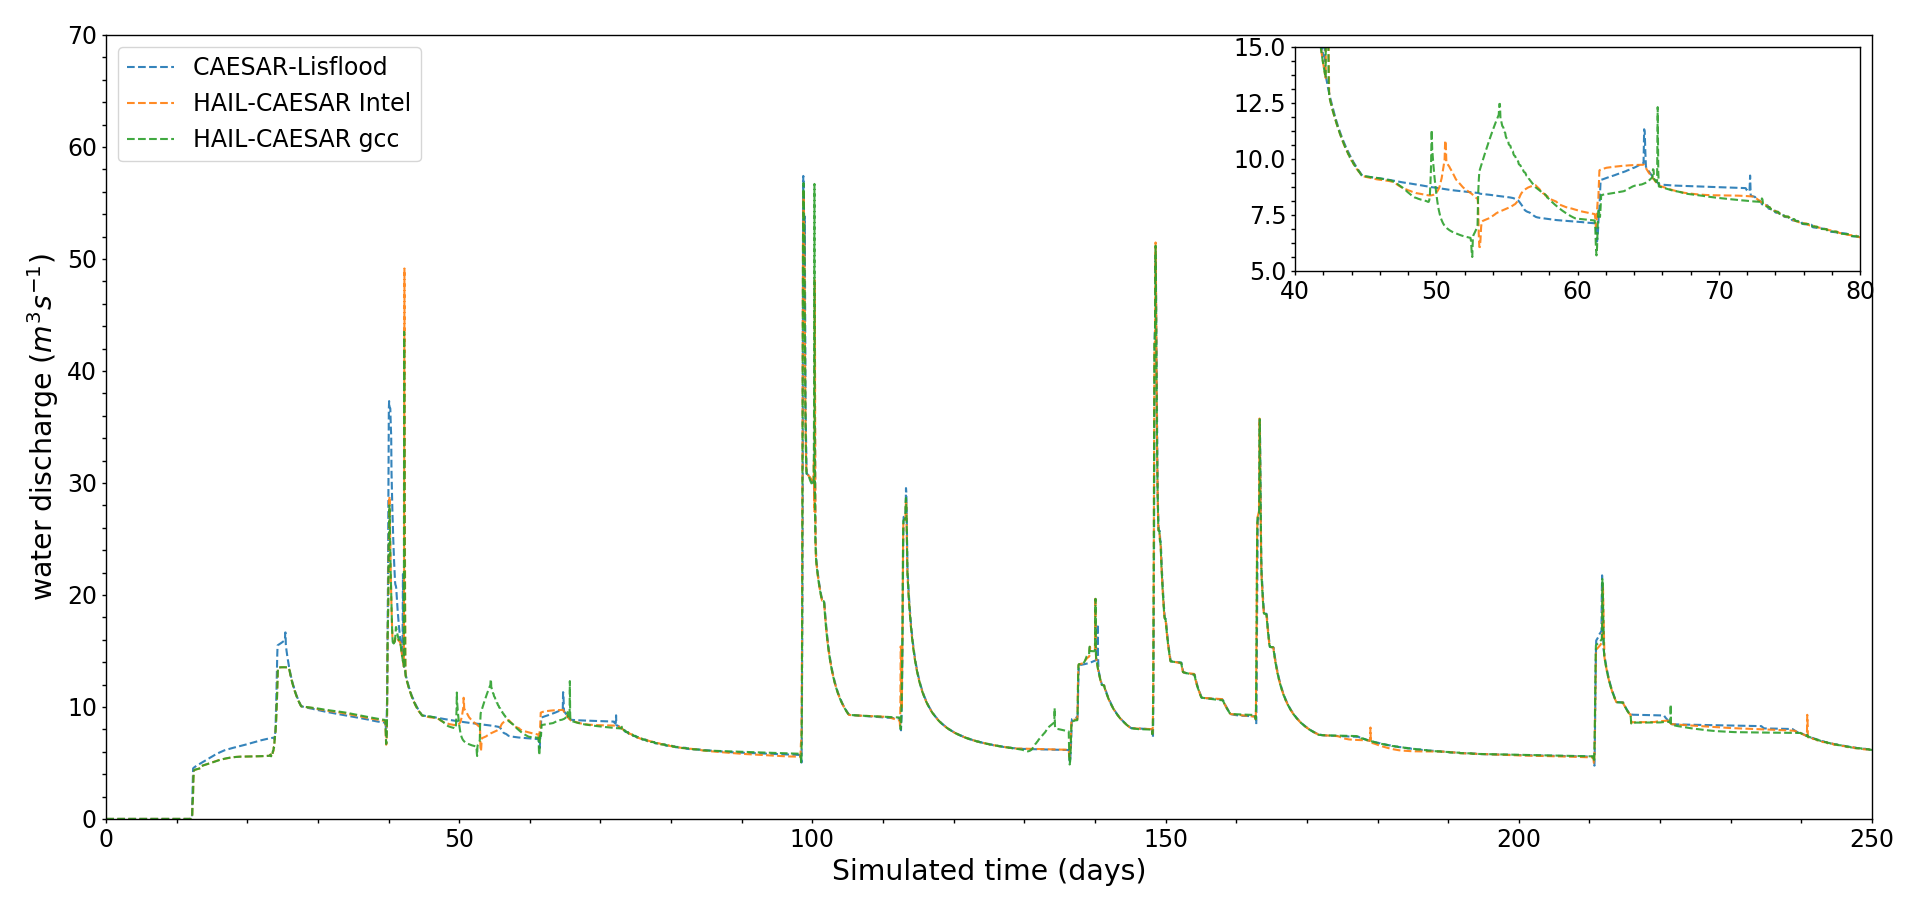
\includegraphics[width=25cm]{chp05_figures_scripts/lisflood_regerssion_new_colours13.png}
\caption{Water discharge rates over first 250 days of simulation. Outputs from the Swale 10 year at 50m resolution test case, showing results from the original CAESAR-Lisflood model and HAIL-CAESAR model compiled under two different compilers: Intel and GCC.}
\label{fig_swale_regression_lisflood}
\end{sidewaysfigure*}

\begin{sidewaysfigure*}[t]
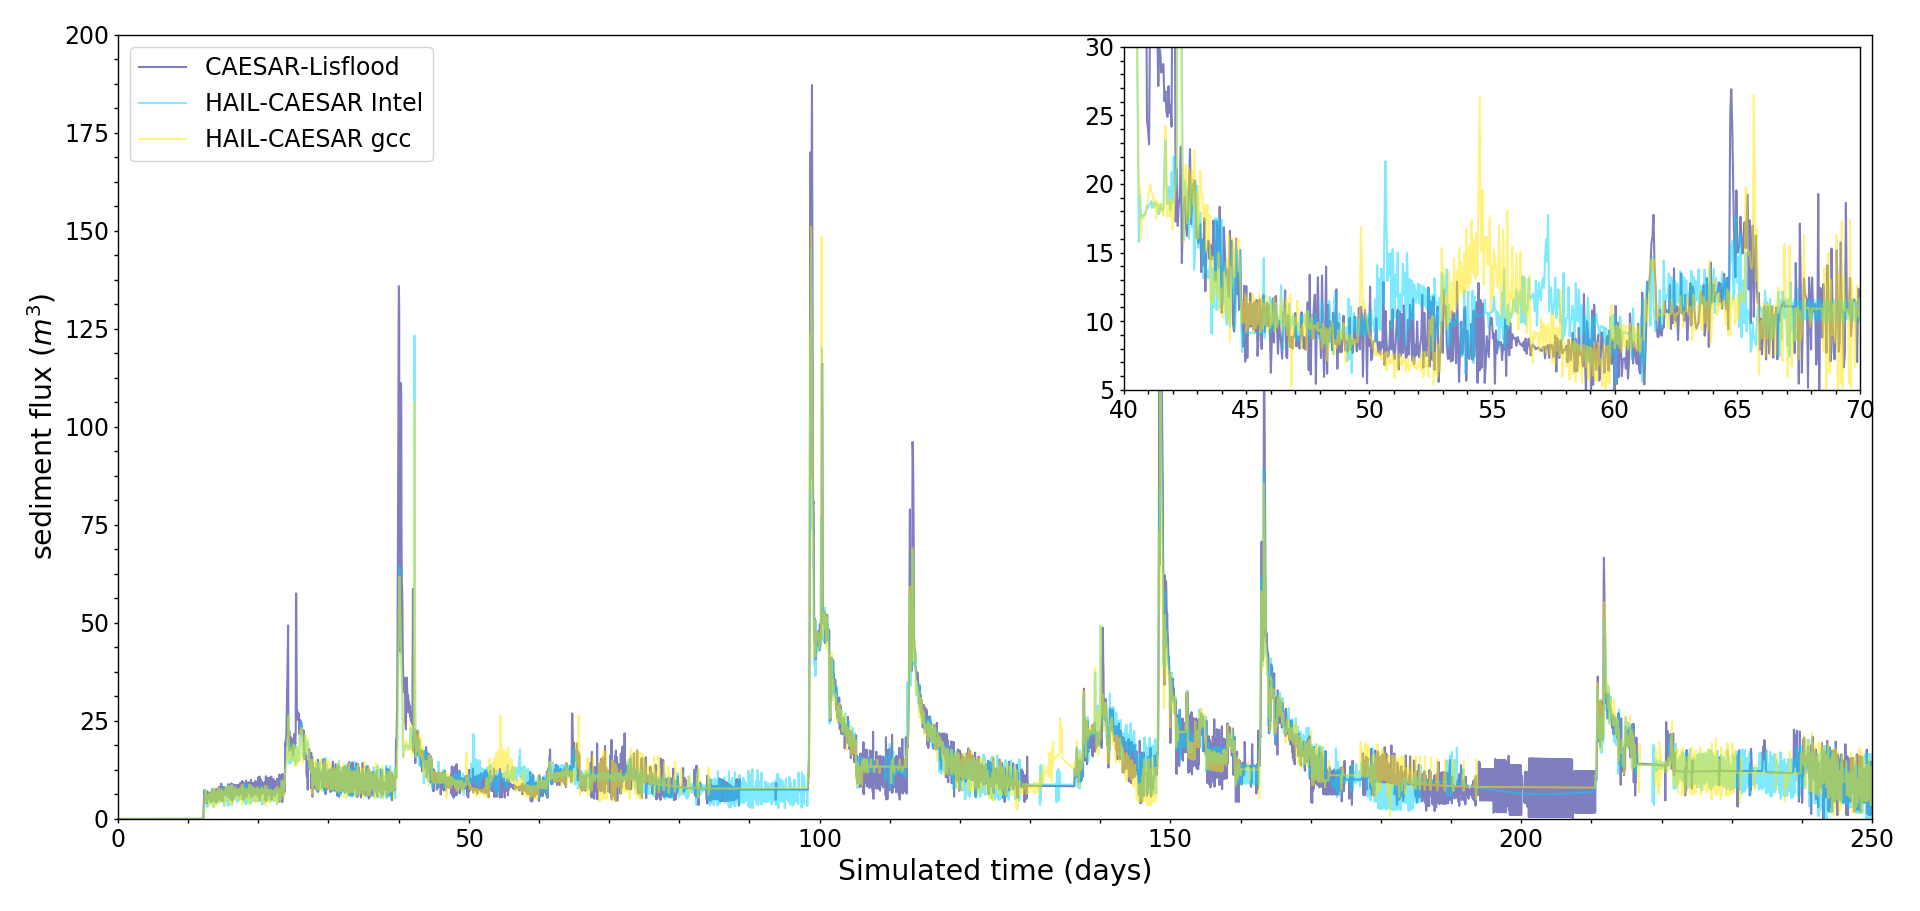
\includegraphics[width=25cm]{chp05_figures_scripts/sed_tot_regression_alpha.png}
\caption{Catchment sediment flux over first 250 days of simulation. Outputs from the Swale 10 year at 50 m resolution DEM test case, showing results from the original CAESAR-Lisflood model and HAIL-CAESAR model compiled under two different compilers: Intel and GCC.}
\label{fig_swale_regression_sediment}
\end{sidewaysfigure*}

\begin{figure}[t]
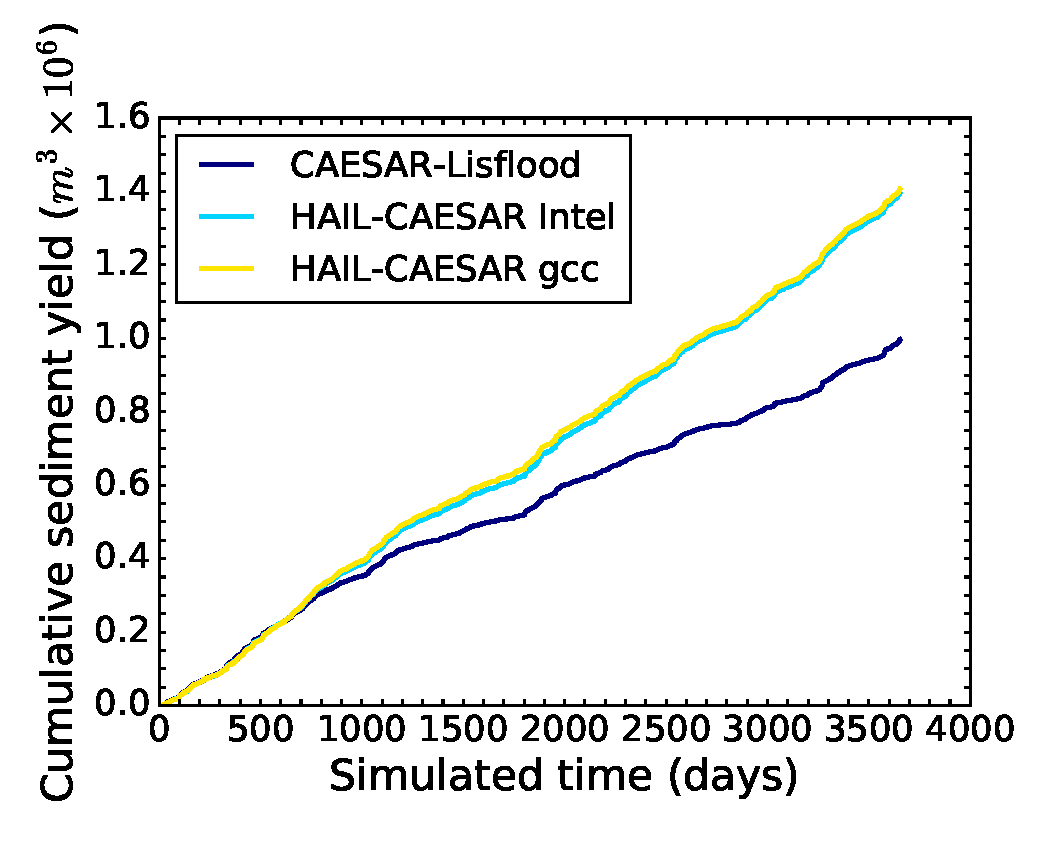
\includegraphics[width=15cm]{chp05_figures_scripts/cum_sed_tot_regression.eps}
\caption{Cumulative catchment sediment flux over full duration of simulation. Outputs from the Swale 10 year at 50 m DEM resolution test case, showing results from the original CAESAR-Lisflood model and HAIL-CAESAR model compiled under two different compilers: Intel and GCC.}
\label{fig_swale_regression_cum_sediment}
\end{figure}

\subsection{Performance comparison with CAESAR-Lisflood}

Though the code base of HAIL-CAESAR and CAESAR-Lisflood differ somewhat, due to differences in implementation detail between the C\# and C++ languages, as well as the parallelisation libraries used, the underlying algorithms remain broadly the same. The two models were compared on similar hardware to assess any gains in speed-up from porting the CAESAR-Lisflood model to a C++ implementation using the OpenMP parallelisation libraries.

The hardware used for this test study was a workstation computer with an Intel i7 8-core processor and 32GiB of memory. The CAESAR-Lisflood test simulations were run on a Windows operating system, as per the requirements of the software; the HAIL-CAESAR model test simulations were run on a Linux operating system on the same machine. The input parameters and input DEM were kept the same for all benchmarking simulations. The details of the test case configurations are shown in Table \ref{versus_CL}.

Using the HAIL-CAESAR implementation, a speed up of c.41\% was seen using the open-source GNU C++ compiler (gcc) and a speed-up of 48\% using the Intel C++ compiler. As the core algorithms remain the same in both versions of the code, the speed up likely comes from the fewer overheads in the command-line based HAIL-CAESAR model, and potentially through better compiler optimisations available with the C++ compilers. Further speed up may come from the fact that the CAESAR-Lisflood model is executed through a \textit{just-in-time} compiler, translating pre-compiled bytecode into machine code at runtime \citep{aycock2003brief}. In contrast, HAIL-CAESAR runs using a compiled binary executable file, with machine code generated at compile time. The HAIL-CAESAR approach avoids the potential overheads of invoking the dynamic compilation stage in C\#/.NET programs.

\begin{table*}


\resizebox{\textwidth}{!}
{%
\begin{tabular}{cccc}
%\multicolumn{4}{c}{} \\
Model Version & \textbf{CAESAR-Lisflood 1.9b} & \multicolumn{2}{c}{\textbf{HAIL-CAESAR v1.0}} \\
\hline \\
Runtime (hrs:mins) & 7:00 & 4:09 & 3:39 \\
Programming Language & C\# & C++ & C++ \\
Compiler & MSVC 14.0 & GCC 6.2 & Intel v17.0 \\
Optimisation flags & -optimize & -O3, -march=native & -O3, -march=native \\
Parallel library & C\# native parallel library & OpenMP 4.5 & OpenMP 4.0 \\
Processor & \multicolumn{3}{c}{Intel i7-3770 8 core @ 3.4GHz, 32GiB memory} \\
\hline \\
\end{tabular} 
}
\caption{Initial performance and compilation comparison with CAESAR-Lisflood, using the River Swale test case, 50m DEM, 10 year simulation} 
\label{versus_CL}
\end{table*}

\subsection{HPC profiling and speed-up}

\subsection{Performance scaling on HPC compute nodes}
Our primary aim in developing this software was to have a code that ran on Unix-based high performance computing systems and could be re-compiled for a variety of different platforms and computer architectures. This section demonstrates the scaling potential and optimal hardware configurations using a single compute node on a typical HPC system. Test simulations are run on the ARCHER supercomputer. Each compute node consists of a two Intel Ivybridge Xeon processors, each with 12 cores per physical processor. Simultaneous multi-threading allows each core on the processor to effectively act as if it were two separate processing units, giving a total of 48 possible threads/cores per compute node. A single compute node consists of two NUMA\footnote{Non-uniform memory access}-regions each with access to 16GiB of memory, a total of 32GiB per compute node. 

\subsection{Strong scaling}
Strong scaling describes how the performance increase of the code scales as more processors are used to solve a problem of fixed size. We test two typical use case scenarios for the HAIL-CAESAR model. The first case is an extension of the standard test case using the Swale data. The use of the model in this case is typical of longer duration landscape evolution simulations, with periods of predominantly low hydrological flows interspersed with brief (relative to the simulation time) storm events. The second case uses the HAIL-CAESAR model to simulate a single storm event at higher spatial resolutions, over a much shorter timescale. Two contrasting model applications are chosen to represent the range of timescales the model can be applied to, from short term single storm events to annual and decadal simulations. 

\begin{table}
\caption{Strong scaling test cases used to benchmark the HAIL-CAESAR model, using Swaledale and Boscastle DEMs.}
\begin{tabular}{ccccc}
\\
\multicolumn{5}{c}{\textbf{Strong scaling benchmarking simulations}} \\
\hline 
Catchment & Swaledale & \multicolumn{3}{c}{Boscastle} \\
Grid cells & 124931 & \multicolumn{2}{c}{720000} & 4500000 \\ 
DEM cell size & 50m & 5m & 5m & 2m \\ 
Simulation time & 8670 hrs & 48 hrs & 72 hrs & 72 hrs \\ 
Catchment Size & 150km$^2$ & {12km$^2$} & {12km$^2$} & {12km$^2$} \\ 
Number of cores & \multicolumn{4}{c}{1, 2, 4, 8, 16, 20, 30, 36, 40, 48} \\ 
\hline \\
\end{tabular} 
\label{strong_scale_table}
\end{table}

\paragraph*{Multi-event simulation, 1 year}
The Swaledale test case is run over a 1 year duration, using an input DEM of 50 m resolution. The model is run in hydrology-only and erosion-enabled modes. The input parameters and input DEM are the same for each simulation, as each simulation is repeated on an increasing number of processors (Table \ref{strong_scale_table}). At the maximum core count of 48 core, results from this simulation show speed up of up to 700\% and 550\%, for erosion-enabled and hydrology-only modes, respectively. The speed-up shown for erosion-enabled simulations does not always increase in concert as core-counts are increased, although the overall trend is one of increasing speed-up. For example, erosion-enabled simulations with 16, 24, and 36 processors showed a slow down when compared to the preceding benchmark tests using 12, 20, and 30 processors, respectively (Figure \ref{fig_strong_scale_multi}). The hydrological-only simulations showed a more consistent speed-up between benchmark tests (Fig. \ref{fig_strong_scale_multi}), though speed-up potential begins to decline at thread counts around 30 threads and higher, where it is observed the gains from increasing the thread count further diminish.

\paragraph*{Single-event simulation, 48--72 hours}

For this benchmark, two sets of strong scaling experiments are done with two different resolution DEMs. For each set of experiments, the input terrain data and parameters remain the same while increasing the number of processors over which the problem is shared. The strong scaling benchmark tests use a model domain with a) 720 000 grid cells, and b) 4 500 000 grid cells, representing a 12km$^2$ river catchment with 5m and 2m resolution DEMs, respectively. At this resolution of DEM, it possible to resolve the larger channel geometries at the grid-scale, without resorting to techniques of `burning in' the DEM with a channel. Sub-grid parameterisation of the channel shape, a feature of some models, is also not required.

Since HAIL-CAESAR features both a flood-inundation-only and sediment erosion mode, two further sets of benchmarks were done for both problem sizes, one with the model running in hydrology-only mode, and another running in the erosion-enabled mode.

The results from the single-event scaling benchmark show the greatest speed-up for the 48 hour Boscastle simulation, with a speed-up of almost 16 times at 48 threads/cores, for the hydrology-only simulation. Erosion-enabled simulations also show food speed-up for this problem size (720 000 grid cells), but the linear speed-up trend is lost above around 30 cores, when speed-up gains begin to tail-off. At the larger problem size of 4 500 000 grid cells, the speed-up gains from increasing core counts is much diminished, though still increases linearly through higher core counts. Speed-up here reaches only about 5 times running on 48 cores, in hydrology-only mode, and 3.5 times in erosion-enabled mode.

\begin{figure}[t]
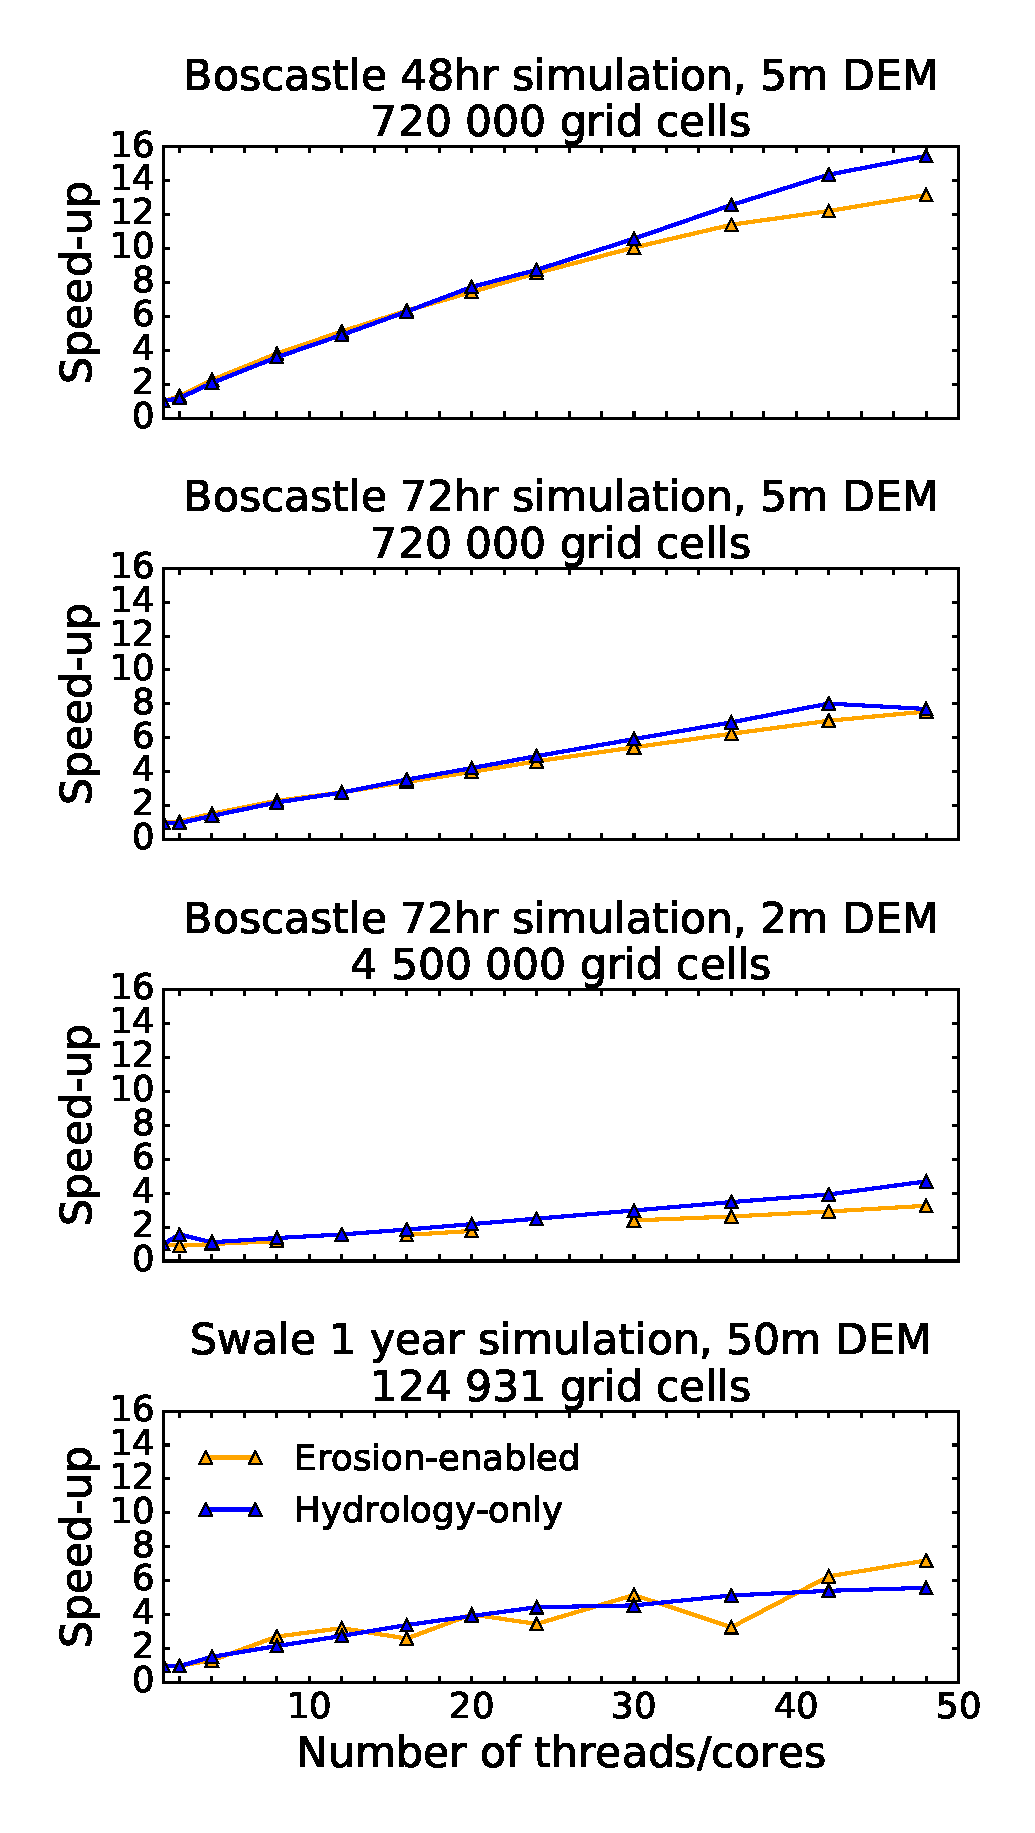
\includegraphics[width=11cm]{chp05_figures_scripts/strong_scale_four.eps}
\caption{Speed-up achieved relative to serial code on 2, 4, 8, 12, 16, 20, 24, 30, 36, 42, and 48 cores. Four sets of simulations are used representing a range of model uses from short, single event episodes (48--72hr) to 1 year simulations.}
\label{fig_strong_scale_multi}
\end{figure}

\subsection{Weak scaling}

Weak scaling is a parallel performance metric used to assess how the code runtime scales as the amount of work per processor is kept the same, but the total problem size -- in our case, the number of grid cells in the model domain -- is increased \citep{gustafson1988reevaluating}. This mirrors the practice of using larger numbers of processors to tackle model simulations using higher resolution topographic data, or data covering a larger spatial domain. The weak scaling experiments used a set of hydrology-only simulations and a set of erosion-enabled simulations. A series of 72 hour simulations were done using a range of high-resolution topographic datasets, from 0.5 m to 5 m resolution, scaling the number of processors used to maintain the ratio of processors/workload as near as possible. The number of model domain grid cells per core was fixed at approximately 1 500 000. The simulations were repeated for hydrological-mode and erosion-enabled modes, but due to the high memory demands of running very high resolution erosion-enabled simulations, not all simulations could be completed on the available hardware, which has a maximum job runtime of 48 hours.

The simulations in hydrological-only mode show positive weak scaling as the problem size increases in tandem with the number of threads (Figure \ref{fig_weak_scale}). Ideal weak scaling would be expected to show a runtime per number of grid cells/cores remaining approximately constant compared with a single-threaded simulation. The slight increase seen in the weak scaling here is likely due to the overheads experienced with creating and synchronising the extra threads as the problem size is increased.

\begin{sidewaystable*}[t]
\caption{Weak scaling test cases with the Boscastle DEM resampled at increasing resolutions from 0.5m to 5m. The absence of run-time results for certain erosion simulations is due to memory limitations preventing higher resolution simulations from running.}
\resizebox{\textwidth}{!}
{%
\begin{tabular}{ccccccc}

\multicolumn{7}{c}{\textbf{Weak scaling simulations, Boscastle DEM, 72 hour simulation}} \\ 

DEM resolution (m)  &  Grid cells & Ideal no. of threads & No. of threads & Cells per thread & Run time (Hydro) & Run time (Erosion) \\ 
\hline
0.5 & 72 000 000 & 48    & 48 &  1 500 000 & 323.1 & --  \\
0.6 & 49 900 050 & 33.3 & 33 &  1 512 122 & 190.4 & -- \\
0.7 & 36 808 200 & 24.5 & 26 &  1 472 328 & 138.8 & -- \\
1.0 & 18 000 000 & 12    & 12 &  1 500 000 & 84.3 & 355.2 \\
1.5 & 7 960 050   & 5.3   &  5  &   1 592 010 & 49.0 & -- \\
2.0 & 4 500 000   & 3      &  3  &   1 500 000 & 568.9 & 1112.1 \\
5.0 & 720 000      & 0.48 & 1  &    720 000 & 347.306 & 432.3 \\ 
\hline \\
\end{tabular} 
}
\label{weak_scale_table}
\end{sidewaystable*}

\begin{figure}[t]
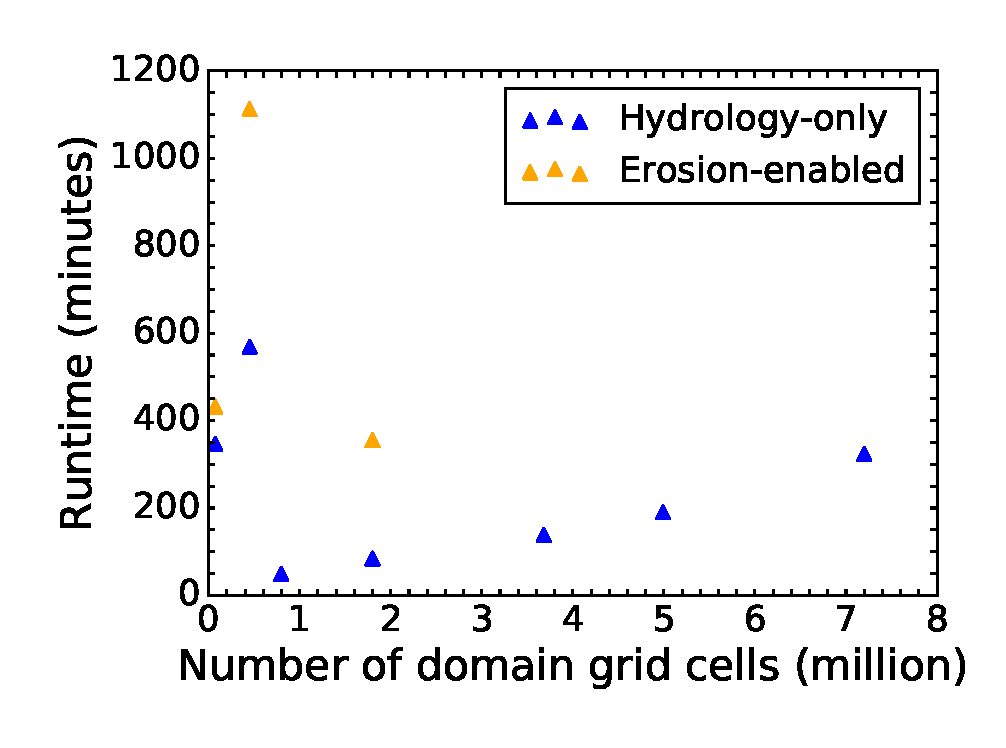
\includegraphics[width=11cm]{chp05_figures_scripts/weak_scale_bos.eps}
\caption{Weak scaling with the Boscastle DEM at increasing resolution (see Table \ref{weak_scale_table}). Hydrological and erosion-enabled simulations shown. Each simulation uses c.150 000 grid cells per CPU. The absence of results for certain erosion simulations is due to memory limitations preventing higher resolution simulations from running.}
\label{fig_weak_scale}
\end{figure}


%\subsubsection{Compiler influence}
%
%The influence of compiler choice on performance is investigated using three compilers: gcc v5.1, Intel vX, and the Cray compiler vX.X.
%
%\subsubsection{Optimisation options}

\subsection{Thread profiling}

Further profiling of the parallelised version of the code was carried out using the Intel\textregistered \ VTune Amplifier performance analyser. Thread profiling allows us to see where the bottlenecks in the code are, including functions that are compute intensive, but also where inefficiencies occur due to overheads from parallelisation and load imbalance. For clarity, a single example using the Boscastle test case is presented, with a simulated model time of 48 hours, running on 8 cores/threads. It is expected that different simulations and domain sizes would produce slightly different results, but this simulation gives a general idea of the parallel performance of specific functions in the code.

The break down of major function overheads is shown in Figure \ref{fig_thread_profile}. Only four of the key parallel-implemented functions, \textit{erode, flow\_route, scan\_area,} and \textit{depth\_update} are assessed, as other functions collectively amounted to a small proportion of the runtime, or were serial functions. Load imbalance accounts for 22\% of the execution time of these four key functions, due to certain threads sitting idle while waiting for other threads to complete. Load imbalance is particularly apparent in the \textit{erode} and \textit{depth\_update} functions. Overhead time (from the creation and synchronisation of threads) is minimal across all functions. The issue of load imbalance is discussed further in Section \ref{sec_loadbalance}.

\begin{figure}[t]
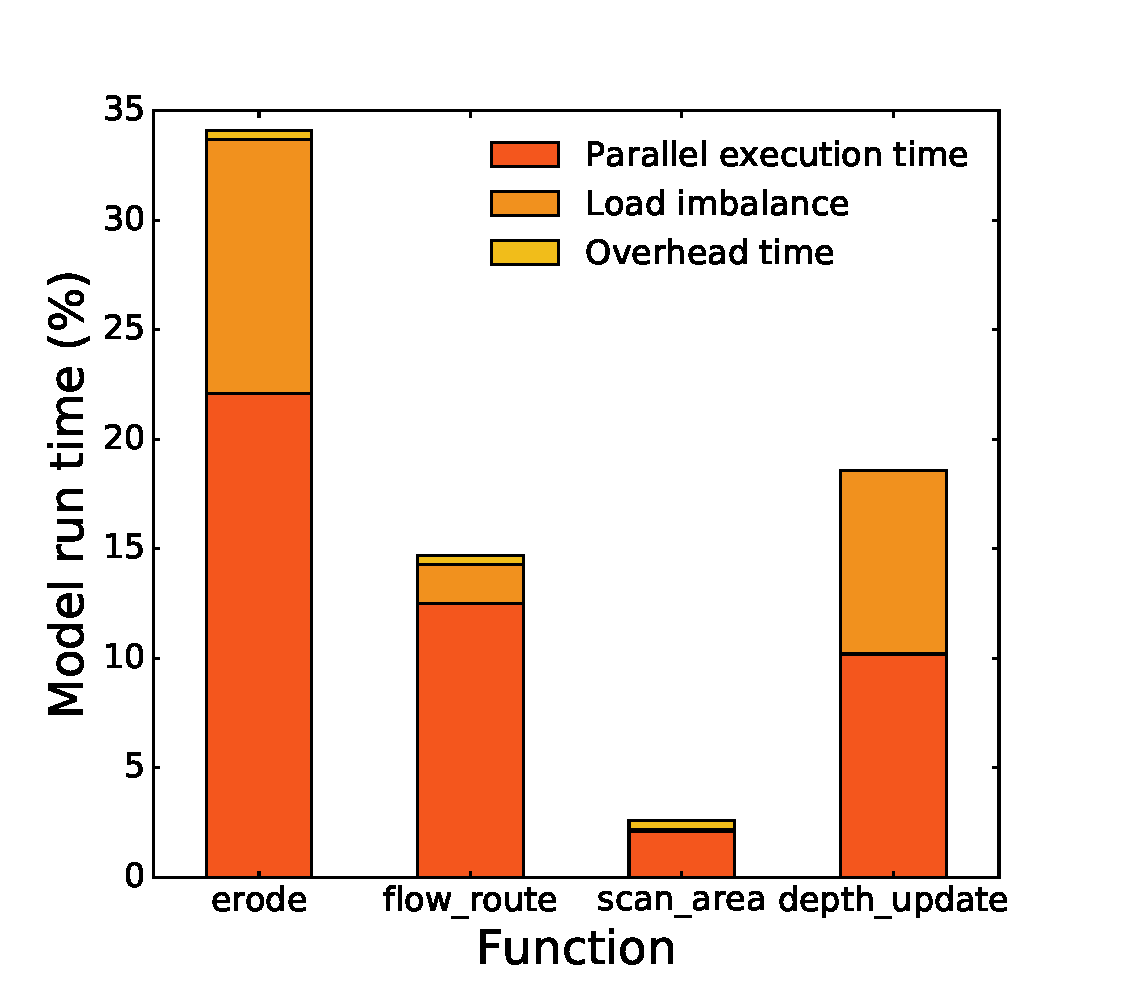
\includegraphics[width=11cm]{chp05_figures_scripts/fig_thread_profile.eps}
\caption{Thread profiling of the Swale 1 year simulation with 50m DEM. Data from major functions only displayed.}
\label{fig_thread_profile}
\end{figure}

%\subsection{Ensemble simulation potential on HPC clusters}
%
%The growing availability of HPC services has been thus far seldom exploited by the geomorphic and landscape evolution modelling community. This section briefly explores the potential for using such computing services to run ensemble simulations of landscape evolution models, using the HAIL-CAESAR model and Swale test case used in previous sections. The ARCHER HPC service is used for the test simulations. 

\section{Discussion}

%Strong scaling
%weak scaling
%Problem-type and size dependency
%Load-balancing issue
%Scheduling

\subsection{Parallel scaling}
%Strong scaling
%weak scaling
%Problem-type and size dependency
There are three factors that potentially affect the parallel scaling observed in the benchmarking test cases presented. 
\begin{enumerate}
\item The number of grid cells in a model domain, i.e. the total problem size, which is dependent on the resolution of the DEM input data. 
\item The choice of running the simulation as hydrology-only or erosion-enabled model. The erosion option in the model also increases memory demands significantly compared to the hydrology-only mode, as well as computational expense.
\item The hydrological state of the catchment. When the catchment is experiencing flooding due to high rates of rainfall input, the number of cells registered as containing water through the \textit{scan\_area} algorithm increases substantially. The location of the water-containing cells in a catchment also determines the amount of load-imbalance in the model. If water-containing cells are concentrated only in a certain area of the catchment, significant load-imbalance will occur. 
\end{enumerate}

The most favourable speed-up was observed in the Boscastle 48 hour simulation at 5 m DEM resolution (Figure \ref{fig_strong_scale_multi}.) A speed-up of almost 16x was recorded using the maximum number of cores available on the test hardware. Increasing the length and resolution of the Boscastle simulation appeared to negatively affect the speed-up potential of the simulation. Speed-up gains remained approximately linear into higher core counts, with slight tail-off in speed-up gains observed when approaching 48 cores. The longer-term Swale simulation exhibited poorer scaling, with a gradual drop in speed-up gains as the number of threads/cores was increased. 

There is not a clear relationship between number of grid cells in the model domain and speed-up potential. The Swale test case (about 125 000 grid cells), for example, showed almost half as much speed up as the 48 hour Boscastle simulation, despite the latter having 720 000 grid cells in the model domain. 

The enabling of erosional processes in simulations did not significantly affect the scaling potential of the simulations. Most benchmark results showed slightly less favourable speed up at higher core counts for erosion-enabled simulations, but this did not appear to be the controlling factor on scaling. In one case (Swale) the erosion-enabled simulation ran 2x faster than the corresponding hydrology-only simulation. The lack of contrast between erosion-enabled and hydrology-only simulations may be explained by the adpative time stepping feature used in the \textit{erode} function. In erosion-enabled mode, the timestep increases substantially during periods of low water flow and erosion rates, and this may offset the increased computational demands from the \textit{erode} function.

The Boscastle and Swale test cases represent different types of catchment hydrological state. The Boscastle simulations essentially represent a single intense flooding event, where the catchment is in a period of low flow followed by an intense burst of rainfall and erosion for a few hours. The Swale simulation represents a series of storm events, interspersed with `dry' periods, where the model will be able to increase the timestep, but not make heavy use of parallel sections of the code reserved for water routing and erosion routines. 

\subsection{Load balancing issues}
\label{sec_loadbalance}
Parallel computing problems in which the distribution of workload between each thread or processor is uneven are said to suffer from \textit{load-imbalance}. In other words, although the model domain is divided into equally sized chunks for the number of threads and processors available, each thread will not necessarily receive an equal amount of work to do \citep{sakellariou1996quest}. Threads with little amounts of work to do will therefore remain idle while waiting for  heavily-loaded threads complete their assigned work. Numerical simulation of river catchments is inherently load-imbalanced. The load balance problem arises from the nature of catchment processes, where the most rapid rates of geomorphological activity occur in river channels. In river channels, rates of water flow and sediment transport are greatest, relative to the processes operating on hillslopes. The inherent heterogeneity in the nature of catchment processes translates into computational imbalance during model simulations of river catchments. Within the model domain representing a catchment, the grid cells of the domain representing river channel sections will make the greatest computational demand, due to repeated calls to subroutines that calculation or update cell properties. Highly active river channel cells will frequently exceed thresholds set for the calculation of water flows and sediment entrainment, whereas cells representing hillslope areas will be active relatively infrequently.

The mechanism in the model that determines which cells will be updated each iteration is the scanning algorithm described in the \textit{scan\_area} section. The algorithm was originally designed \citep{Coulthard2013} to substantially reduce the number of cells in the model domain that had to be updated each iteration, by isolating the cells that contain water and only performing erosion and sediment transport routines on those `wetted' cells. While the algorithm is effective at reducing compute time this way, it creates a load-imbalance problem for parallel implementations as the location of computationally intensive areas of the model domain cannot be easily predetermined. While threads are assigned equal numbers of iterations, each iteration is not necessarily equally load-balanced in terms of computational expense. In algorithms that perform a global scan of all cells in the model domain, such as the parallel implementation of the flow routing algorithm in \citet{neal2009parallelisation}, load imbalance is minimalised because threads are kept occupied working on every grid cell, rather than focusing on a subset of grid cells with discharge or water depth above a given threshold, as is done in the HAIL-CAESAR model. A global scanning algorithm was initially explored in the implementation of HAIL-CAESAR, allowing the removal of the \textit{scan\_area} function, but the increase in run-time was so substantial it negated any potential improvements in load balance among the OpenMP threads. 

\subsection{Loop scheduling}

The OpenMP application programming interface (API) will automatically partition iterations of a loop between the available number of threads. By default these are assigned statically when a \texttt{parallel for} block is entered, with threads receiving an equal number of loop iterations to carry out. The default behaviour can be overridden, however, by explicitly specifying a different scheduling type for parallel for loops. For load imbalanced problems such as discussed in this paper, the \textit{dynamic} loop scheduling can improve parallel performance by reducing the amount of idle time that threads spend waiting for busy threads to complete their workload \citep{willebeek1993strategies,olivier2012openmp}. The default behaviour of the dynamic scheduling type is to assign each loop iteration to one thread, and when the thread finishes it is assigned the next iteration that has yet to be executed. Experiments in finding an ideal loop scheduling set-up to reduce load imbalance in HAIL-CAESAR showed mixed results, with no clear indication that using the dynamic scheduling clause improved run-times in all cases. However, in some test cases, dynamic loop scheduling was shown to offer performance improvement. For this reason, the HAIL-CAESAR model provides users with the option to set the loop scheduling type at run time, by specifying the \texttt{OMP\_SCHEDULE} environment variable before running the model. It is recommended that users experiment with using dynamic scheduling for their own simulations as it may offer performance increases over default scheduling.



\section{Conclusions}  %% \conclusions[modified heading if necessary]
An implementation of a hydrodynamic landscape evolution model was developed, based on the CAESAR-Lisflood model \citep{Coulthard2013}. The new C++ implementation of the model is modular, cross-platform, and scalable to multi-core computing systems through the implementation of shared-memory parallelism with the OpenMP API. Minimal code changes were required to the serial version of the code to deliver a parallel compute code. The model exhibits a performance increase of c.40\% compared to the CAESAR-Lisflood implementation in a like-for-like benchmark. The scaling potential of the model is variable, depending on the size of the problem domain and the likely hydrological state of the river catchment being simulated. In most test cases, linear speed up is achieved at moderate core counts of up to 48 cores, on model domain sizes of up to 4.5 million grid cells. Computational load imbalance was a substantial problem in the model. The causes of the load balancing issues in the model are likely due to the spatially-heterogeneous nature of catchment-scale hydrological and erosional processes. Suggestions are made for minimising load imbalance through dynamic loop scheduling, but the success of these scheduling methods is highly dependent on the input data to the model.
